{
\chapter[Data augmentation instead of explicit regularisation]{Data augmentation\\instead of explicit regularisation}
\label{ch:daugreg}
\renewcommand{\chapterpath}{includes/daug-reg}
%
\begin{outreach}
    \item \textit{Data augmentation instead of explicit regularization.} \textbf{Alex Hern{\'a}ndez-Garc{\'i}a}, Peter K{\"o}nig. arXiv preprint arXiv:1806.03852, 2018.
    \item \textit{Do deep nets really need weight decay and dropout?.} \textbf{Alex Hern{\'a}ndez-Garc{\'i}a}, Peter K{\"o}nig. arXiv preprint arXiv:1802.07042, 2018.
    \item \textit{Further advantages of data augmentation on convolutional neural networks.} \textbf{Alex Hern{\'a}ndez-Garc{\'i}a}, Peter K{\"o}nig. International Conference on Artificial Neural Networks (ICANN, Best Paper Award), 2018.
\end{outreach}
%
Data augmentation in machine learning refers to the techniques that synthetically create new examples from a data set by applying possibly stochastic transformations on the existing examples. In the image domain, these transformations can be, for instance, slight translations or rotations, which preserve the perceptual appearance of the original images, but significantly alter the actual pixel values. Despite being an old technique \citep{abumostafa1990hints, simard1992daug} and ubiquitous in the deep learning literature and practice, data augmentation has often been regarded as a sort of \textit{cheating}, \textit{lower class} technique\footnote{As a result, the machine learning scientific community has heavily ignored data augmentation as a subject of study until recently. By way of illustration, the textbook Deep Learning \citep{goodfellow2016dlbook} dedicates one and a half pages to data augmentation, of which one third is devoted to the caveats of data augmentation. Only in the last few years has data augmentation started to receive increasing attention, likely due to the success of some data augmentation techniques, such as \textit{cutout} \citep{devries2017cutout} and \textit{mixup} \citep{zhang2017mixup}, and especially by the popularisation by Google of \textit{automatic} data augmentation \citep{cubuk2018autoaugment}, previously proposed by various university groups \citep{hauberg2016learningdaug, antoniou2017dagan, ratner2017learningdaug, lemley2017smartdaug}. We first submitted the results presented in this chapter in 2017 \citep{hergar2018daugregopenreview} and other authors have also presented surveys on data augmentation techniques \citep{perez2017dauganalysis, shorten2019daugsurvey}. Promisingly, very recently has data augmentation started to be analysed as well from a theoretical point of view \citep{rajput2019daug, chen2019invariance, lyle2020daug}}, which should not be used in order to assess the actual strength of a new proposal \citep{goodfellow2013maxout, graham2014fracmaxpool, larsson2016fractalnet, goodfellow2016dlbook}. A common criticism is that data augmentation usually requires domain or expert knowledge and it cannot be easily generalised across data domains \citep{devries2017daugfeatspace}.

Explicit regularisation methods such as weight decay \citep{hanson1989wd} and dropout \citep{srivastava2014dropout} are also nearly ubiquitous. In contrast, they are considered intrinsic parts of the learning algorithm and thus have remained unquestioned. However, in Chapter~\ref{ch:reg}, we have introduced the differences between explicit and implicit regularisation and raised the question of whether explicit regularisation is necessary in deep learning. On the other hand, in the Introduction (Chapter~\ref{ch:intro}) we have discussed the view of data augmentation as a powerful inductive bias from visual perception. Building upong these insights, in this chapter, we analyse the role of data augmentation in neural networks trained for image object categorisation and the need for weight decay and dropout when data augmentation is used. We first derive some theoretical insights from statistical learning theory and then present the results of a large empirical study in which we contrast the contributions of each technique.
%

\section{Theoretical insights}
\label{sec:daugreg-theoretical_insights}
As we have reviewed in Section~\ref{sec:background-generalisation}, the generalisation of a model class $\mathcal{H}$ can be analysed through complexity measures such as the VC-dimension or, more generally, the Rademacher complexity $\mathcal{R}_{N}(\mathcal{H}) = \mathbb{E} \left[ \hat{\mathcal{R}}_{N}(\mathcal{H}) \right]$, where:
%
\begin{equation}
\label{eq:daugreg-rademacher}
  \hat{\mathcal{R}}_{N}(\mathcal{H}) = \mathbb{E}_{\sigma} \left[ \underset{h \in \mathcal{H}}{\mathrm{sup}} \left| \frac{1}{N} \sum_{i=1}^{N} \sigma_{i}h(x_{i}) \right| \right]
\end{equation}
% 
is the empirical Rademacher complexity, defined with respect to a specific set of $N$ data samples. Then, in the case of binary classification and the class of linear separators, the generalisation error of a hypothesis, $\hat{\epsilon}_{N}(h)$, can be bounded using the Rademacher complexity:

\begin{equation}
\label{eq:daugreg-genbound}
 \hat{\epsilon}_{N}(h) \leq \mathcal{R}_{N}(\mathcal{H}) + \mathcal{O} \left( \sqrt{\frac{\ln \sfrac{1}{\delta}}{N}} \right)
\end{equation}
%
with probability $1 - \delta$. Tighter bounds for some model classes, such as fully connected neural networks, can be obtained \citep{bartlett2002rademacher}, but it is not trivial to formally analyse the influence on generalisation of specific architectures or techniques. Nonetheless, we can use these theoretical insights to discuss the differences between explicit regularisation---specifically weight decay and dropout---and data augmentation. 

A straightforward yet very relevant conclusion from the analysis of any generalisation bound is the strong dependence on the number of training examples $N$. Increasing $N$ drastically improves the generalisation guarantees, as reflected by the second term in the right hand side of Equation~\ref{eq:daugreg-genbound} and by the dependence of the Rademacher complexity (Equation~\ref{eq:daugreg-rademacher}) on the sample size too. Data augmentation exploits prior knowledge about the data domain and aspects of visual perception---in the case of image object recognition---to create new examples and its impact on generalisation is related to an increment in $N$, as stochastic data augmentation can generate virtually infinite different samples. Admittedly, the augmented samples are not independent and identically distributed and thus, the effective increment of samples does not strictly correspond to the increment in $N$. This is why formally analysing the impact of data augmentation on generalisation is complex. Recent studies have made progress in this direction by analysing the effect of simple data transformations on generalisation from a theoretical point of view \citep{chen2019invariance, rajput2019daug}.

Explicit regularisation methods aim, in contrast, at improving the generalisation error by constraining the hypothesis class $\mathcal{H}$ to reduce its complexity $\mathcal{R}_{N}(\mathcal{H})$ and, in turn, the generalisation error $\hat{\epsilon}_{N}(h)$. Crucially, while data augmentation exploits domain knowledge, most explicit regularisation methods only \textit{naively} constrain the hypothesis class, by simply reducing the representational capacity, as we have discussed in the previous chapter. For instance, weight decay constrains the learnable models $\mathcal{H}$ by setting a penalty on the weights norm. Interestingly, \citet{bartlett2017boundsnn} showed that weight decay has little impact on the generalisation bounds and confidence margins. Dropout has been extensively used and studied as a regularisation method for neural networks \citep{wager2013dropout}, but the exact way in which it impacts generalisation is still an open question. In fact, it has been stated that the effect of dropout on neural networks is ``somewhat mysterious'', complicated and its penalty highly non-convex \citep{helmbold2017dropout}. Recently, \citet{mou2018dropout} have established new generalisation bounds on the variance induced by a specific type of dropout on feedforward networks. 

An interesting observation is that dropout can be analysed as a random form of data augmentation without domain knowledge \citep{bouthillier2015dropoutasdaug}. This implies that any generalisation bound derived for dropout can be regarded as a pessimistic bound for domain-specific, standard data augmentation. A similar argument applies for weight decay, which, as first shown by \citet{bishop1995tikhonov}, is equivalent to training with noisy examples if the noise amplitude is small and the objective is the sum-of-squares error function. Therefore, some forms of explicit regularisation are at least approximately equivalent to adding random noise to the training examples, which is the simplest form of data augmentation\footnote{Note that the opposite view---domain-specific data augmentation as explicit regularisation---does not apply. In Section~\ref{sec:reg-taxonomies} we discuss about the taxonomies of regularisation, including the difference between data augmentation and data-dependent regularisation}. Thus, it is reasonable to argue that more sophisticated data augmentation can overshadow the benefits provided by explicit regularisation.

In general, we argue that the reason why explicit regularisation may not be necessary is that neural networks are already implicitly regularised by many elements---stochastic gradient descent (SGD), convolutional layers, normalisation and data augmentation, to name a few---that provide a more successful inductive bias \citep{neyshabur2014implicitreg}. For instance, it has been shown that linear models optimised with SGD converge to solutions with small norm, without any explicit regularisation \citep{zhang2016understandingdl}. Furthermore, as discussed in Section~\ref{sec:reg-discussion}, if overparameterised neural networks are able to generalise well, the need for constraining their capacity is questionable. In the rest of the chapter we present an empirical study to contrast data augmentation and explicit regularisation---weight decay and dropout.

\section{Methods}
\label{sec:daugreg-methods}
This section describes the main aspects of the experimental setup for systematically analysing the role of data augmentation in deep neural networks compared to weight decay and dropout.

\subsection{Data}
\label{sec:daugreg-methods_data}
We performed the experiments on the highly benchmarked data sets ImageNet \citep{russakovsky2015imagenet} ILSVRC 2012, CIFAR-10 and CIFAR-100 \citep{krizhevsky2009cifar}. We resized the 1.3 M images from ImageNet into $150\times200$ pixels, as a compromise between keeping a high resolution and speeding up the training. Both on ImageNet and on CIFAR, the pixel values were mapped into the range $[0, 1]$.  

So as to analyse the role of data augmentation, we trained every model with two different augmentation schemes as well as with no data augmentation at all. The two augmentation schemes are the following:

\subsubsection{\textit{Light} augmentation}
This scheme is common in the literature, for example \citep{goodfellow2013maxout, springenberg2014allcnn}, and performs only horizontal flips and horizontal and vertical translations of 10\% of the image size. 

\subsubsection{\textit{Heavier} augmentation}
This scheme performs a larger range of affine transformations such as scaling, rotations and shear mappings, as well as contrast and brightness adjustment. On ImageNet we additionally performed random crops of $128\times128$ pixels. The choice of the allowed transformations is arbitrary and the only criterion was that the objects be still recognisable in general. We deliberately avoided designing a particularly successful scheme. The details of the transformations are presented below and the range of the parameters are specified in Table~\ref{tab:daugreg-heavier_params} and some visual examples are shown in Figure~\ref{fig:daugreg-cifar10_daug}.

\begin{itemize}
  \item Affine transformations: 
  \vspace{5pt} \\
    $
      \begin{bmatrix}
      x^\prime \\
      y^\prime \\
      1
      \end{bmatrix}
      = 
      \begin{bmatrix}
      f_h z_x \cos(\theta) & -z_y \sin(\theta + \phi) & t_x \\
      z_x \sin(\theta) & z_y \cos(\theta + \phi) & t_y \\
      0 & 0 & 1
    \end{bmatrix}
    \begin{bmatrix}
      x \\
      y \\
      1
      \end{bmatrix}
    $
  \item Contrast adjustment: $x^\prime = \gamma (x - \overline{x}) + \overline{x}$

  \item Brightness adjustment: $x^\prime = x + \delta$
\end{itemize}

\begin{table}[ht]
\begin{center}
\begin{tabular}{cll}
\textbf{Parameter} & \textbf{Description}   & \textbf{Range}                                            \\
\hline \\
$f_h$              & Horiz. flip        & $1 - 2 B(0.5)$                                            \\
$t_x$              & Horiz. translation & $\mathcal{U}(-0.1, 0.1)$                                  \\
$t_y$              & Vert. translation   & $\mathcal{U}(-0.1, 0.1)$                                  \\
$z_x$              & Horiz. scale       & $\mathcal{U}(0.85, 1.15)$                                 \\
$z_y$              & Vert. scale         & $\mathcal{U}(0.85, 1.15)$                                 \\
$\theta$           & Rotation angle         & $\mathcal{U}(-22.5^\circ, 22.5^\circ)$  \\
$\phi$             & Shear angle            & $\mathcal{U}(-0.15, 0.15)$                                \\
$\gamma$           & Contrast               & $\mathcal{U}(0.5, 1.5)$                                   \\
$\delta$           & Brightness             & $\mathcal{U}(-0.25, 0.25)$                                
\end{tabular}
\end{center}
\caption{Description and range of possible values of the parameters used for the heavier augmentation scheme. $B(p)$ denotes a Bernoulli distribution and $\mathcal{U}(a, b)$ a uniform distribution.}
\label{tab:daugreg-heavier_params}
\end{table}

\begin{figure}[htb]
  \begin{center}
    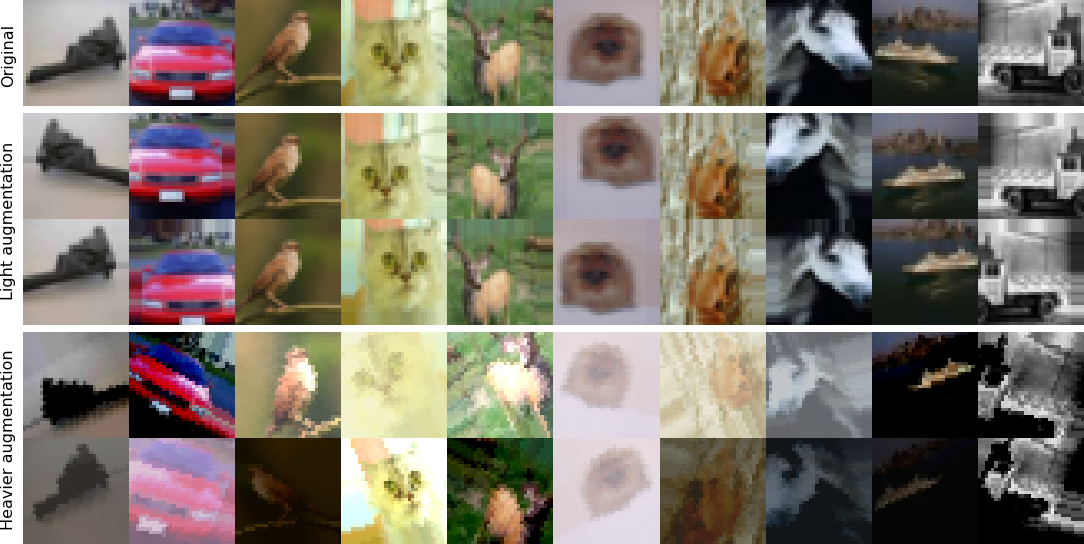
\includegraphics[width = \textwidth]{\imgpath/cifar10_daug}
  \end{center}
  \caption{Illustration of the most extreme transformations performed by the data augmentation schemes on ten images---one per class---from CIFAR-10.}
  \label{fig:daugreg-cifar10_daug}
\end{figure}

\subsection{Network Architectures}
\label{sec:daugreg-methods_archs}
We trained three distinct, popular architectures that have achieved successful results in visual object recognition: the all convolutional network, All-CNN \citep{springenberg2014allcnn}; the wide residual network, WRN \citep{zagoruyko2016wrn}; and the densely connected network, DenseNet \citep{huang2017densenet}. Importantly, we kept the training hyperparameters---learning rate, training epochs, batch size, optimiser, etc.---as in the original papers. Table~\ref{tab:architectures} summarises the main features of each network and below we specify further details.

\begin{table}[ht]
\begin{center}
\begin{tabular}{rccc}
    & \textbf{All-CNN} & \textbf{WRN} & \textbf{DenseNet}\\
    Ref. in original paper & \textit{All-CNN-C} & \textit{WRN-28-10} & \textit{DenseNet-BC}\\
    Main feature & Only conv. layers & Residual connections & Dense connectivity\\
    Number of layers & 16 / 12 & 28 & 101\\
    Number of parameters & 9.4 / 1.3 M & 36.5 M & 0.8 M\\
    Training hours & 35--45 / 2.5 & 100--145 / 14--15  & 24--27\\
\end{tabular}
\end{center}
\caption{Key aspects of the network architectures. Cells with two values correspond to ImageNet  / CIFAR.}
\label{tab:architectures}
\end{table}

\subsubsection{All Convolutional Network}
All-CNN consists exclusively of convolutional layers with ReLU activation \citep{glorot2011relu}, it is relatively shallow and has few parameters. For ImageNet, the network has 16 layers and 9.4 million parameters; for CIFAR, it has 12 layers and about 1.3 million parameters. In our experiments to compare the adaptability of data augmentation and explicit regularisation to changes in the architecture (Section~\ref{sec:daugreg-depth}), we also tested a \textit{shallower} version, with 9 layers and 374,000 parameters, and a \textit{deeper} version, with 15 layers and 2.4 million parameters. The four architectures can be described as in Table~\ref{tab:allcnn}, where $K$\textbf{C}$D$($S$) is a $D \times D$ convolutional layer with $K$ channels and stride $S$, followed by batch normalisation and a ReLU non-linearity. \textit{N.Cl.} is the number of classes and Gl.Avg. refers to global average pooling. 

\begin{table}[ht]
\begin{center}
\begin{tabular}{l|l}
\multirow{1}{*}{ImageNet}  & 96\textbf{C}11(2)--96\textbf{C}1(1)--96\textbf{C}3(2)--256\textbf{C}5(1) \\
                           & --256\textbf{C}1(1)--256\textbf{C}3(2)--384\textbf{C}3(1) \\
                           & --384\textbf{C}1(1)--384\textbf{C}3(2)--1024\textbf{C}3(1) \\
                           & --1024\textbf{C}1(1)--\textit{N.Cl}.C1(1) \\
                           & --Gl.Avg.--Softmax \\ [3pt]
\multirow{1}{*}{CIFAR}     & ~2$\times$96\textbf{C}3(1)--96\textbf{C}3(2)--2$\times$192\textbf{C}3(1) \\
                           & --192\textbf{C}3(2)--192\textbf{C}3(1)--192\textbf{C}1(1) \\
                           & --\textit{N.Cl}.C1(1)--Gl.Avg.--Softmax \\ [3pt]
\multirow{1}{*}{Shallower} & ~2$\times$96\textbf{C}3(1)--96\textbf{C}3(2)--192\textbf{C}3(1) \\
                           & --192\textbf{C}1(1)--\textit{N.Cl}.C1(1)--Gl.Avg.--Softmax \\ [3pt]
\multirow{1}{*}{Deeper}    & ~2$\times$96\textbf{C}3(1)--96\textbf{C}3(2)--2$\times$192\textbf{C}3(1) \\
                           & --192\textbf{C}3(2)--2$\times$192\textbf{C}3(1)--192\textbf{C}3(2) \\
                           & --192\textbf{C}3(1)--192\textbf{C}1(1) \\
                           & --\textit{N.Cl}.C1(1)--Gl.Avg.--Softmax \\
\end{tabular}
\end{center}
\caption{Specification of the All-CNN architectures.}
\label{tab:allcnn}
\end{table}

The CIFAR network is identical to the All-CNN-C architecture in the original paper, except for the introduction of the batch normalisation layers. The ImageNet version also includes batch normalisation layers and a stride of 2 instead of 4 in the first layer to compensate for the reduced input size. 

Importantly, we kept the same training parameters as in the original paper in the cases they were reported. Specifically, the All-CNN networks were trained using stochastic gradient descent, with fixed Nesterov momentum 0.9, learning rate of 0.01 and decay factor of 0.1. The batch size for the experiments on ImageNet was 64 and we trained during 25 epochs decaying the learning rate at epochs 10 and 20. On CIFAR, the batch size was 128, we trained for 350 epochs and decayed the learning rate at epochs 200, 250 and 300. The kernel parameters were initialised according to the Xavier uniform initialisation \citep{glorot2010glorot}.

\subsubsection{Wide Residual Network}
WRN is a modification of ResNet \citep{he2016resnet} that achieves better performance with fewer layers, but more units per layer. Here, we chose for our experiments the WRN-28-10 version (28 layers and about 36.5 M parameters), which was reported to achieve the best results on CIFAR. It has the following architecture:

\begin{center}
\centering
16\textbf{C}3(1)--4$\times$160\textbf{R}--4$\times$320\textbf{R}--4$\times$640\textbf{R}--BN--ReLU--Avg.(8)--FC--Softmax
\end{center}
%
where $K$\textbf{R} is a residual block with residual function  BN--ReLU--$K$\textbf{C}3(1)--BN--ReLU--$K$\textbf{C} 3(1). BN is batch normalisation, Avg.(8) is spatial average pooling of size 8 and FC is a fully connected layer. On ImageNet, the stride of the first convolution is 2. The stride of the first convolution within the residual blocks is 1 except in the first block of the series of 4, where it was set to 2 in order to subsample the feature maps. 

Similarly, we kept the training parameters of the original paper: we trained with SGD, with fixed Nesterov momentum 0.9 and learning rate of 0.1. On ImageNet, the learning rate was decayed by 0.2 at epochs 8 and 15 and we trained for a total of 20 epochs with batch size 32. On CIFAR, we trained with a batch size of 128 during 200 epochs and decayed the learning rate at epochs 60, 120 and 160. The kernel parameters were initialised according to the He normal initialisation \citep{he2015he}.

\subsubsection{DenseNet}

The main characteristic of DenseNet \citep{huang2017densenet} is that the architecture is arranged into blocks whose layers are connected to all the layers below, forming a dense graph of connections, which permits training very deep architectures with fewer parameters than, for instance, ResNet. Here, we used a network with bottleneck compression rate $\theta = 0.5$ (DenseNet-BC), growth rate $k = 12$ and 16 layers in each of the three blocks. The model has nearly 0.8 million parameters. The specific architecture can be described as follows:

\begin{center}
\centering
2$\times k$\textbf{C}3(1)--DB(16)--TB--DB(16)--TB--DB(16)--BN--Gl.Avg.--FC--Softmax
\end{center}
%
where DB($c$) is a dense block, that is a concatenation of $c$ convolutional blocks. Each convolutional block is a set of layers whose output is concatenated with the input to form the input of the next convolutional block. A convolutional block with bottleneck structure has the following layers:

\begin{center}
\centering
BN--ReLU--4$\times k$\textbf{C}1(1)--BN--ReLU--$k$\textbf{C}3(1)--Concat.
\end{center}

TB is a transition block, which downsamples the size of the feature maps, formed by the following layers:

\begin{center}
\centering
BN--ReLU--$k$\textbf{C}1(1)--Avg.(2).
\end{center}

Like with All-CNN and WRN, we kept the training hyperparameters of the original paper. On the CIFAR data sets, we trained with SGD, with fixed Nesterov momentum 0.9 and learning rate of 0.1, decayed by 0.1 on epochs 150 and 200 and training for a total of 300 epochs. The batch size was 64 and the parameters were initialised with He initialisation.

\subsection{Train and Test}
Every architecture was trained on each data set both with explicit regularisation---weight decay and dropout as specified in the original papers---and without. Furthermore, we trained each model with the three data augmentation schemes: no augmentation, light and heavier. The performance of the models was computed on the held out test tests. As in previous works \citep{krizhevsky2012alexnet, simonyan2014}, we averaged the softmax posteriors over 10 random \textit{light} augmentations, since slightly better results are obtained. Then we computed the classification accuracy for the models trained on CIFAR and the top-5 accuracy for the ImageNet models.

All the experiments were performed on Keras \citep{chollet2015keras} on top of TensorFlow \citep{tensorflow2015}, with a single GPU NVIDIA GeForce GTX 1080 Ti.

\section{Results}
\label{sec:daugreg-results}
Here we present the results of the empirical study. In the first set of experiments (Section~\ref{sec:daugreg-orig}) we trained the architectures as in the original papers with the full data sets. A relevant characteristic of explicit regularisation methods is that they typically require the specification of hyperparameters. These are usually fine-tuned by the authors of research papers to achieve higher performance, as demanded by the dynamics of the scientific publication environment in the machine learning community. However, the sensitivity of the results towards these hyperparameters is often not made available. In order to gain insight on the role of explicit regularisation and data augmentation in more real world cases, where the hyperparameters have not been highly optimised, we varied the amount of training data (Section~\ref{sec:daugreg-less_data}) and the depth of the architectures (Section~\ref{sec:daugreg-depth}), while keeping all other hyperparameters untouched.

The objective of the study is to contrast the performance gained by training the models with both explicit regularisation and data augmentation, which is the common practice in the literature \citep{tan2019efficientnet, huang2017densenet, zagoruyko2016wrn, springenberg2014allcnn}, against training with only data augmentation. Hence, the presentation of the results in the figures aims at facilitating this comparison. In the performance plots (bar plots), we represent the relative performance gain of each model with respect to the relevant baseline, which we specify at each section. We plot the results in pairs: the top, purple bars correspond to the models trained with only data augmentation and the bottom, red bars to the models trained with both data augmentation and explicit regularisation. Additionally, we show the results of training with different levels of data augmentation in three colour shades.

In order to assess the statistical significance of the differences between models trained with and without explicit regularisation, we carried out percentile bootstrap analyses \citep{efron1992bootstrap}, that is simulations based on sampling with replacement. We followed the guidelines by \citep{rousselet2019bootstrap}. In all cases, the values of the distribution correspond to the difference between the performance---with respect to the baseline---of the models trained without explicit regularisation minus the performance of the models trained with explicit regularisation. We then compared the distribution of this difference in the bootstrap samples and with respect to the null hypothesis, that is no difference ($H_0 = 0$). For each experiment we sampled all possible bootstrap samples with replacement or a maximum of one million.

\subsection{Original architectures}
\label{sec:daugreg-orig}
%
\begin{figure}[htb]
  \begin{center}
    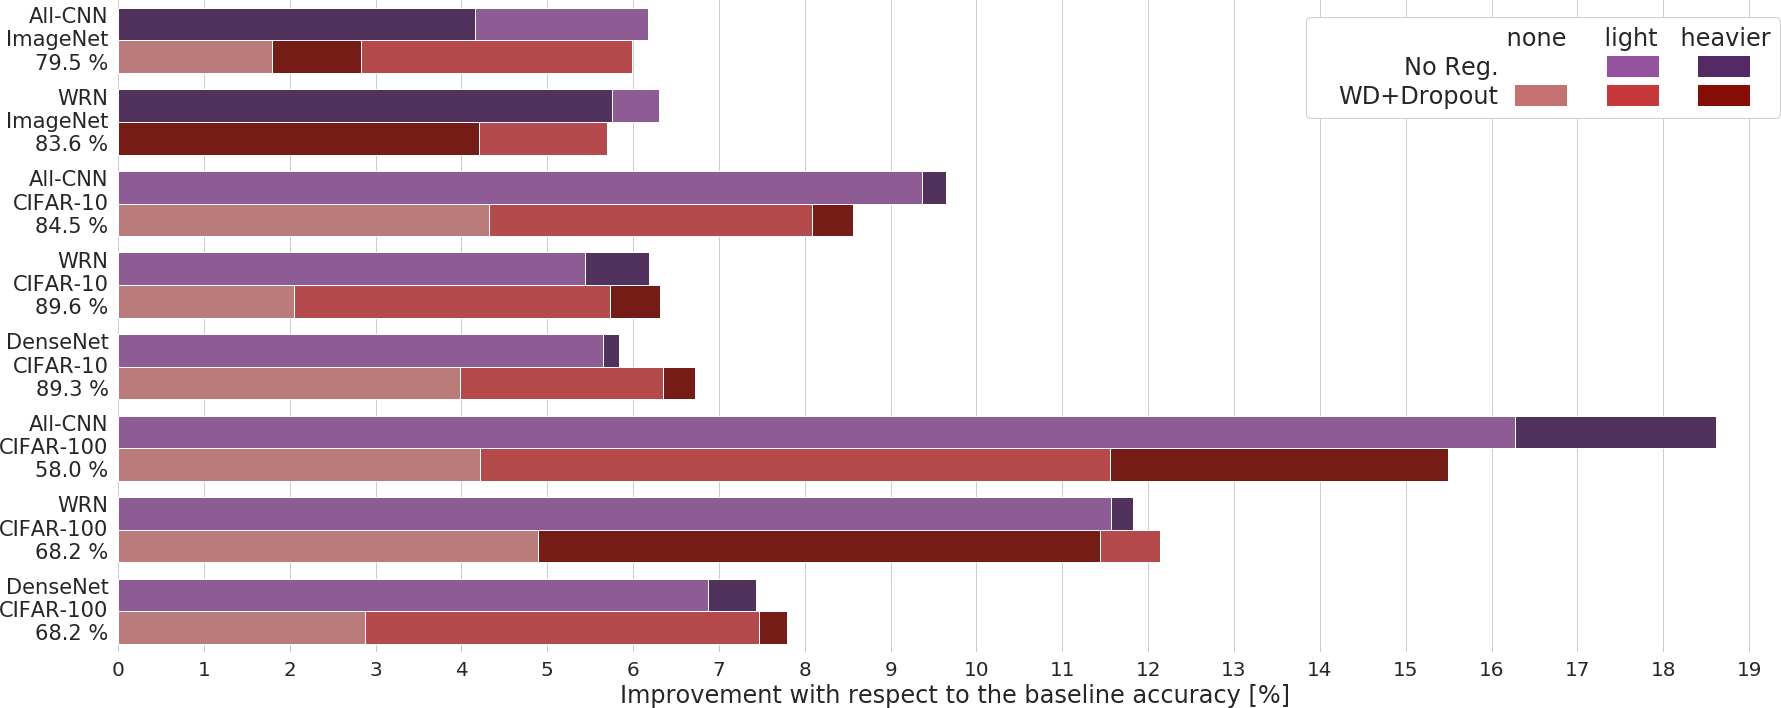
\includegraphics[width = \textwidth]{\imgpath/orig.png}
  \end{center}
  \caption{Relative improvement of adding data augmentation and explicit regularisation to the baseline models, $(accuracy - baseline)/accuracy * 100$. The baseline accuracy is shown on the left. The results suggest that data augmentation alone (purple bars) can achieve even better performance than the models trained with both weight decay and dropout (red bars).}
  \label{fig:daugreg-orig}
\end{figure}

First, we contrast the regularisation effect of data augmentation and weight decay and dropout on the original networks trained with the complete data sets, and show the results in Figure~\ref{fig:daugreg-orig}. As a baseline, we consider the ``bare bone'' models, that is the model trained with neither explicit regularisation nor data augmentation. We report the accuracy of the baseline on the left of the bars in in Figure~\ref{fig:daugreg-orig}. To assess the relevant comparisons, we show the relative improvement in test performance achieved by adding each technique or combination of techniques to the baseline model. Table~\ref{tab:daugreg-orig_nets} shows the mean and standard deviation of each combination on the architecture and data set and Figure~\ref{fig:daugreg-bootstrap_orig} the results of the bootstrap analysis, which considers the differences of all pairs of purple minus red bars\footnote{The relative performance of WRN on ImageNet trained with weight decay and dropout with respect to the baseline is negative (-6.22~\%) and is neither depicted in Figure~\ref{fig:daugreg-orig} nor taken into consideration to compute the average improvements in Table~\ref{tab:daugreg-orig_nets} and the bootstrap analysis in Figure~\ref{fig:daugreg-bootstrap_orig}.}.

\begin{figure}[ht]
  \centering
  \begin{center}
    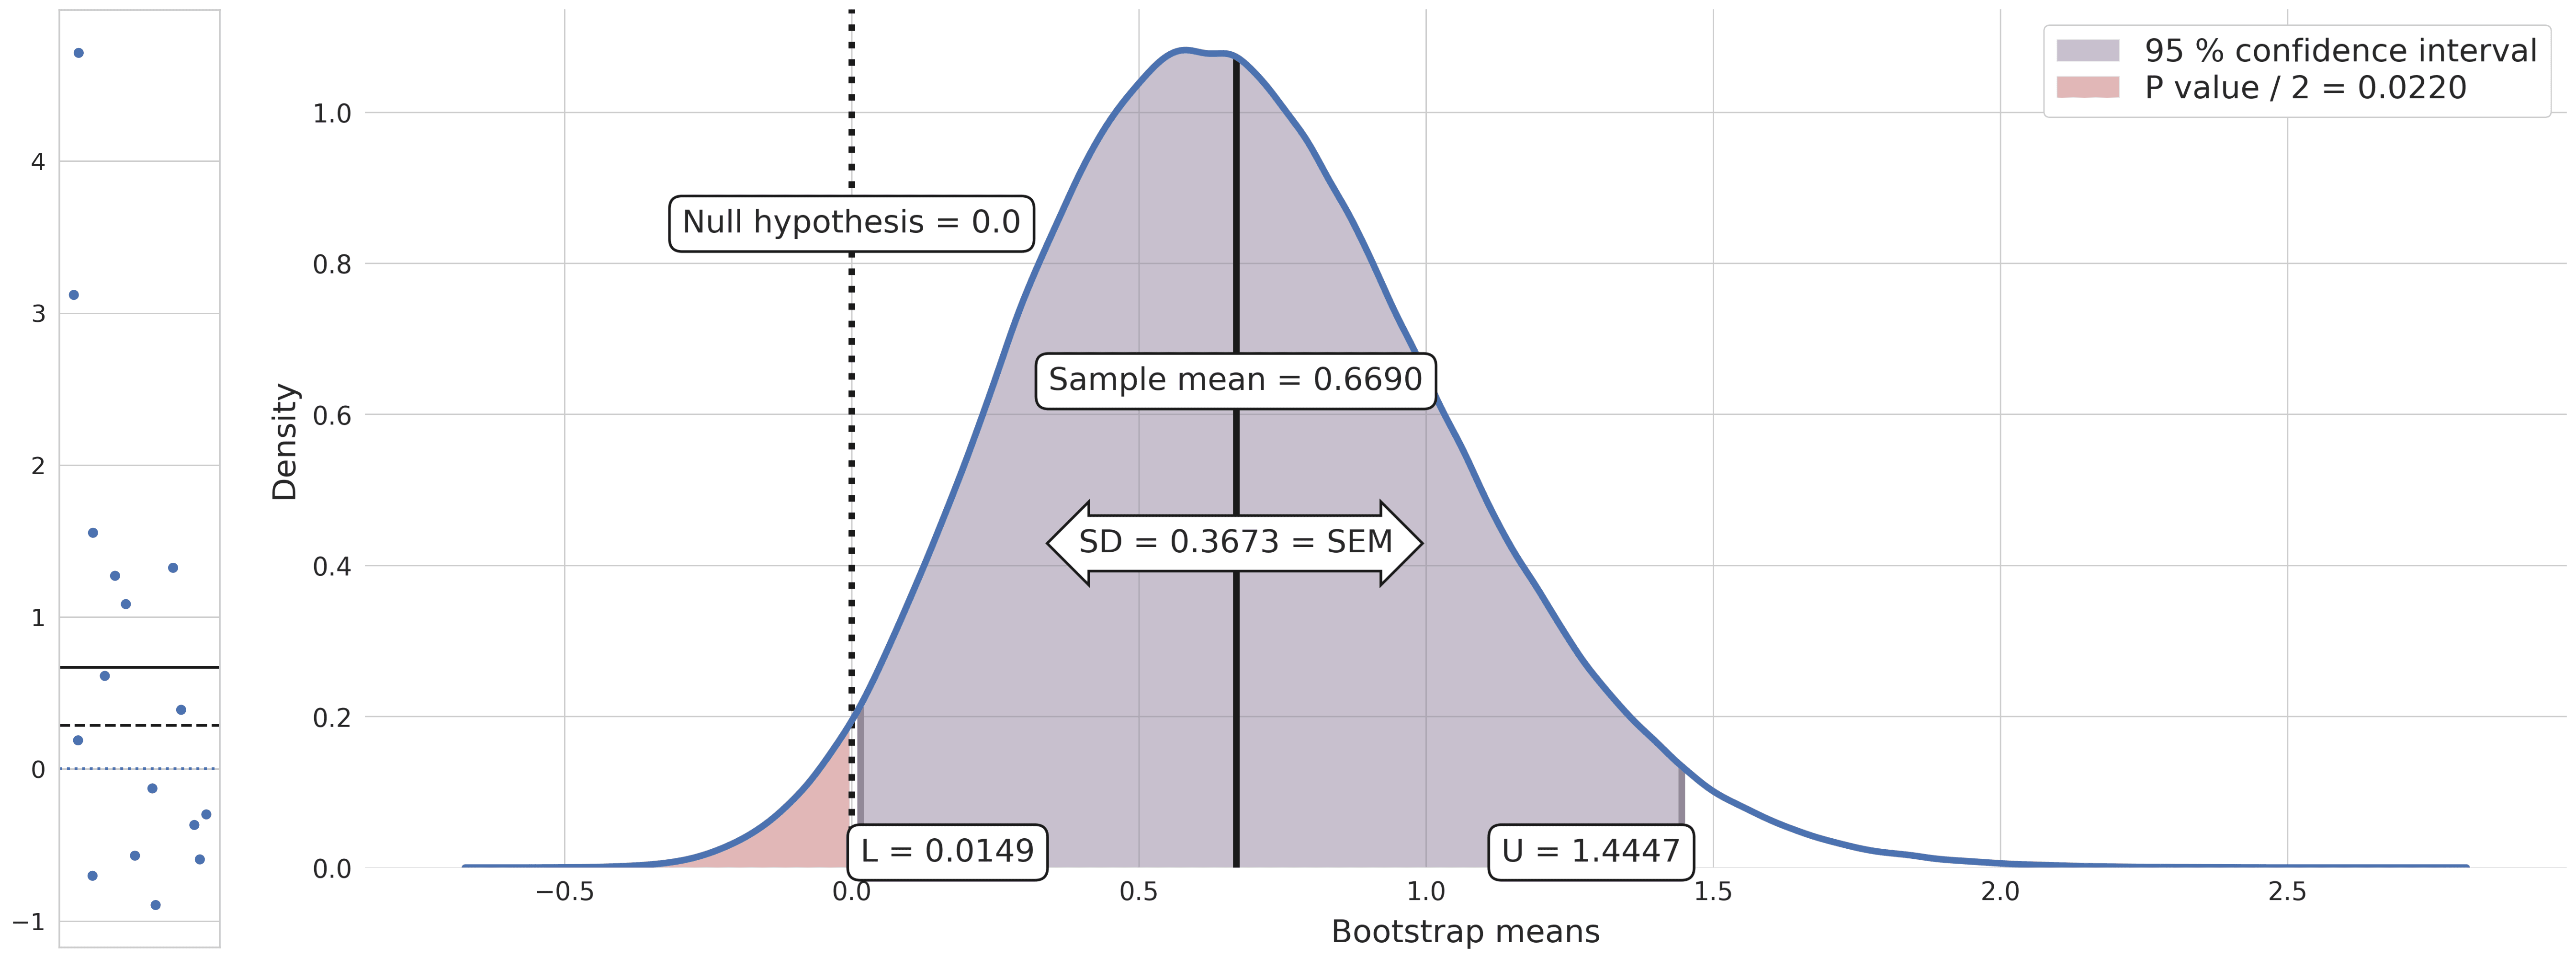
\includegraphics[width = \textwidth]{\imgpath/bootstrap_orig.png}
  \end{center}
  \caption{Bootstrap analysis to assess the difference in performance gain provided by training without and with weight decay and dropout, on the original architectures and using the full data sets. On the left of the figure we plot the bootstrap values---differences---with the mean and median as a solid and dashed line, respectively. The main figure shows the distribution of the mean of the bootstrap samples, the standard error of the sample mean, the 95~\% confidence intervals and the $P$ value with respect to the null hypothesis ($H_0=0$).}
  \label{fig:daugreg-bootstrap_orig}
\end{figure}

\begin{table}[hb]
\begin{center}
\begin{tabular}{rcc}
            & No explicit reg.  & Weight decay + dropout \\
    None    & \textit{baseline} & 3.02 (1.65)            \\
    Light   & 8.46 (3.80)       & 7.88 (2.60)            \\
    Heavier & 8.68 (4.69)       & 7.92 (4.03) 
\end{tabular}
\end{center}
\caption{Average accuracy improvement over the baseline model of each combination of data augmentation level and presence of weight decay and dropout.}
\label{tab:daugreg-orig_nets}
\end{table}

The first conclusion from Figures~\ref{fig:daugreg-orig} and \ref{fig:daugreg-bootstrap_orig} as well as Table~\ref{tab:daugreg-orig_nets} is that training with data augmentation alone (top, purple bars) is better than training with both augmentation and explicit regularisation (bottom, red bars). This is the case in more than half of the cases (9/16) and the bootstrap analysis reveals that the difference is positive with 95~\% confidence and $P$ value $=0.0220$. On average, adding data augmentation to the baseline model improved the accuracy on 8.57~\%, and adding both augmentation and explicit regularisation on 7.90~\% respectively.

At first glance, one may think that this is not remarkable, since the differences are small and data augmentation alone is not better in 100~\% of the cases. However, this result is surprising and remarkable for the following reason: note that the studied architectures achieved state-of-the-art results at the moment of their publication and the models included all light augmentation, weight decay and dropout, whose parameters were presumably finely tuned to optimise the accuracy. The replication of these results corresponds to the middle red bars in Figure~\ref{fig:daugreg-orig}. Here, we have show that simply removing weight decay and dropout---while keeping all other hyperparameters intact, see Section~\ref{sec:daugreg-methods_archs}---improves the \textit{then state-of-the-art} accuracy in 4 of the 8 studied cases. Why did not the authors trained without explicit regularisation and obtain better results?

Second, it can also be observed that the regularisation effect of weight decay and dropout, an average improvement of 3.02~\% with respect to the baseline, is much smaller than that of data augmentation: simply applying light augmentation increased the accuracy in 8.46~\% on average. Although the heavier augmentation scheme was deliberately not designed to optimise the performance, in both CIFAR-10 and CIFAR-100 it improved the test performance with respect to the light augmentation scheme. This was not the case on ImageNet, probably due to the larger complexity of the data set. 

\begin{figure}[htb]
  \begin{center}
    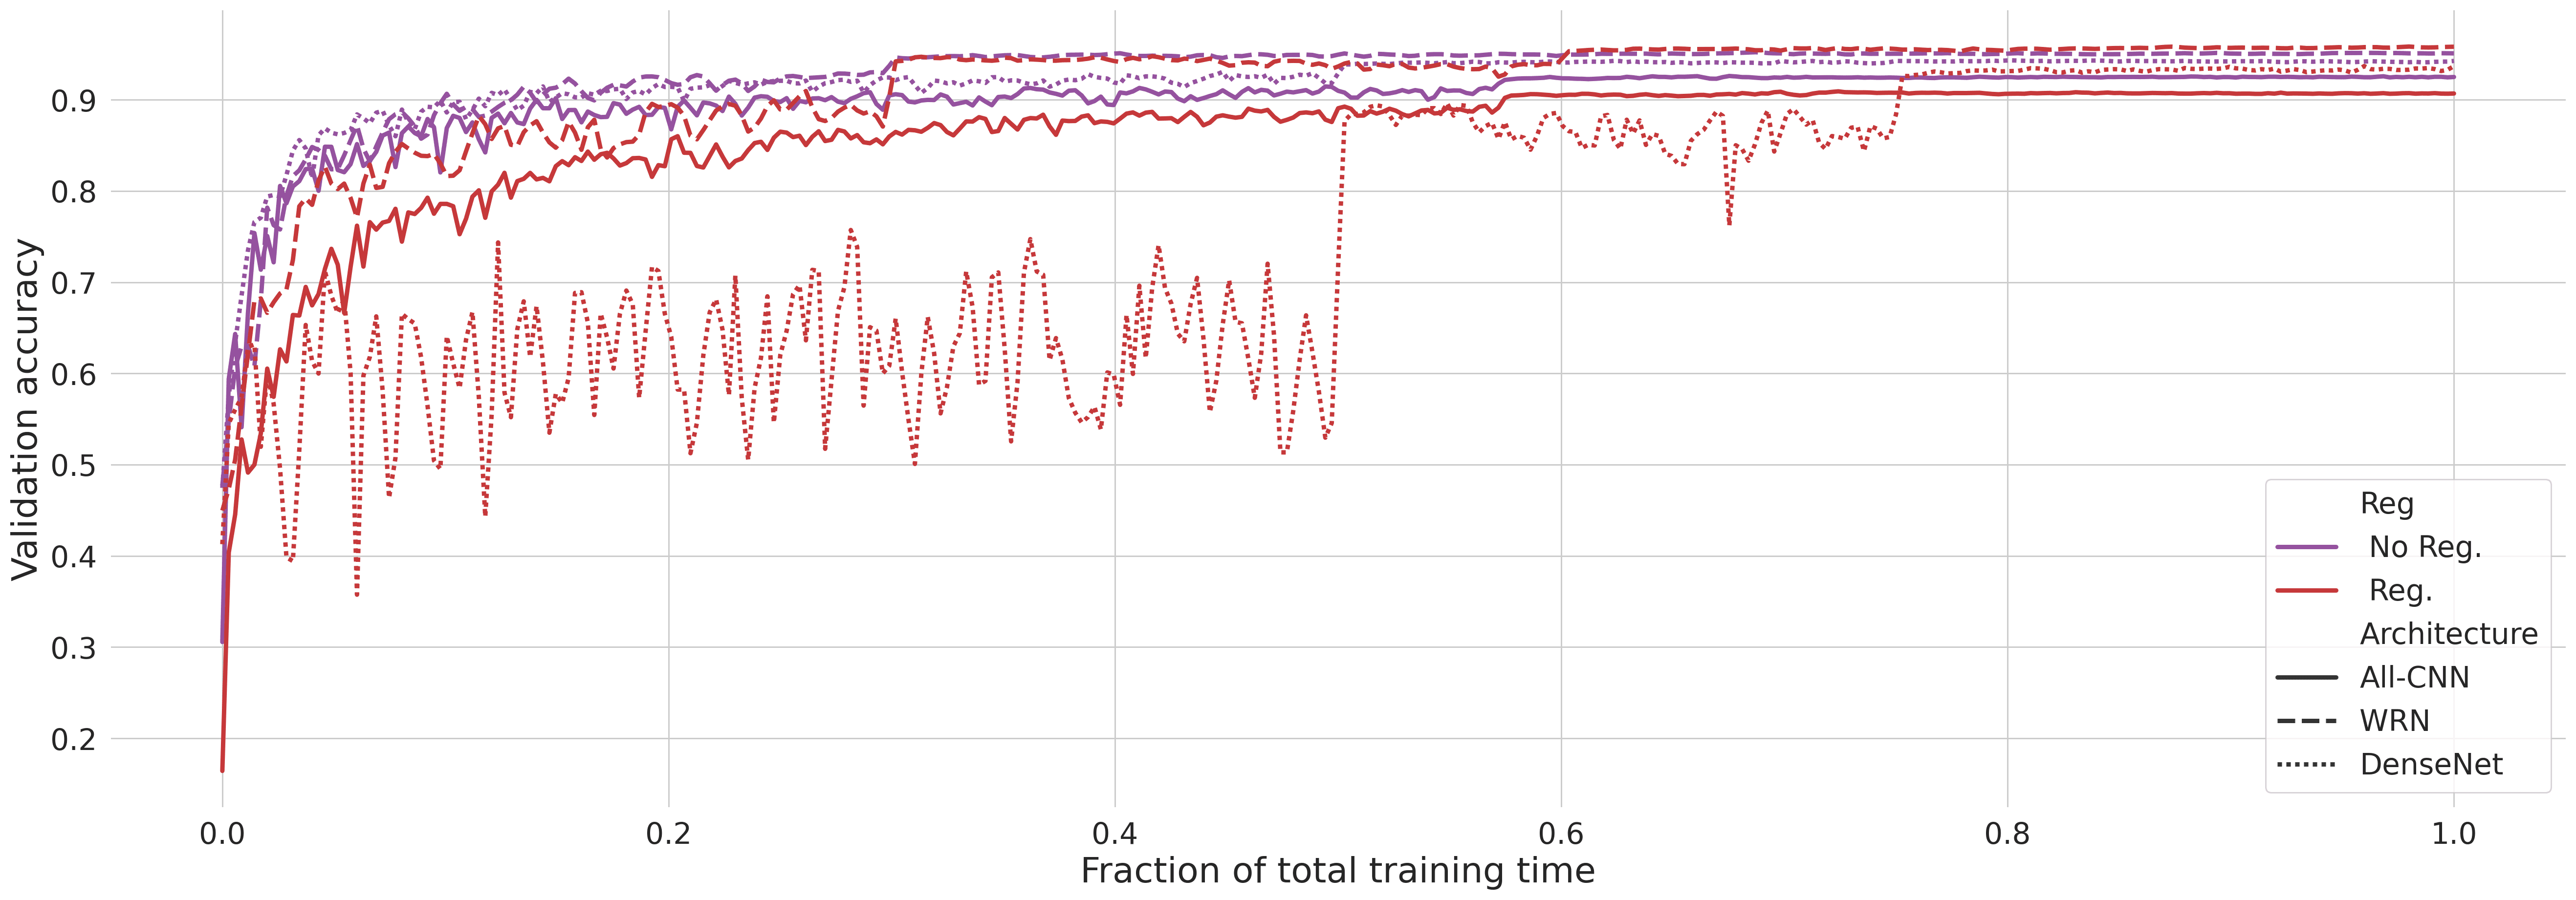
\includegraphics[width = \textwidth]{\imgpath/val_acc_all.png}
  \end{center}
  \caption{Dynamics of the validation accuracy during training of All-CNN, WRN and DenseNet, trained on CIFAR-10 with heavier data augmentation, contrasting the models trained with explicit regularisation (red lines) and the models trained with only data augmentation (purple). The regularised models heavily rely on the learning rate decay to obtain the boost of performance, while the models trained without explicit regularisation quickly approach the final performance.}
  \label{fig:daugreg-dynamics}
\end{figure}

Further, it can be observed that the results are in general more consistent in the models trained without explicit regularisation. Finally, an additional advantage of training without explicit regularisation is that the learning dynamics (Figure~\ref{fig:daugreg-dynamics}) is much faster and predictive of the final performance. Typically, regularisers such as weight decay and dropout effectively prevent the model from fitting the training data during the first epochs and heavily rely on the learning rate decay to obtain the boost that yields the final performance. On the contrary, models trained with only data augmentation reach very high validation performance after a few epochs. This effect is particularly acute on DenseNet, which performs heavier weight decay.

In sum, it seems the performance gain provided by weight decay and dropout can be achieved and often improved by data augmentation alone. Besides, the models trained without explicit regularisation presented additional advantages, which we will further discuss in Section~\ref{sec:daugreg-discussion}.

\subsection{When the available training data changes}
\label{sec:daugreg-less_data}
\begin{figure}[ht]
  \centering
  \begin{subfigure}{\linewidth}
      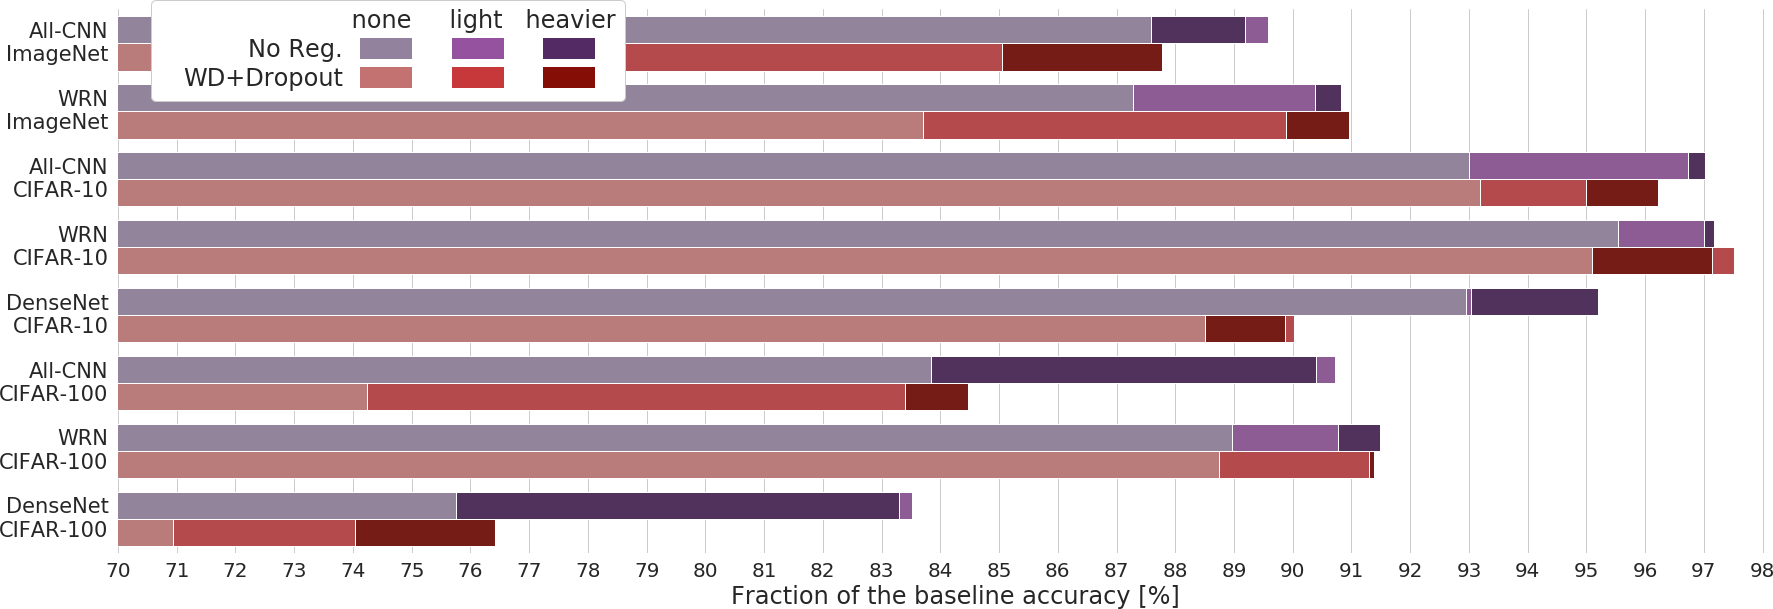
\includegraphics[keepaspectratio=true, width=\columnwidth]{\imgpath/reduced_data_50.png}
      \caption{50~\% of the available training data}
	  \label{fig:daugreg-less_data_50}
  \end{subfigure}
  \\ 
  \begin{subfigure}{\linewidth}
      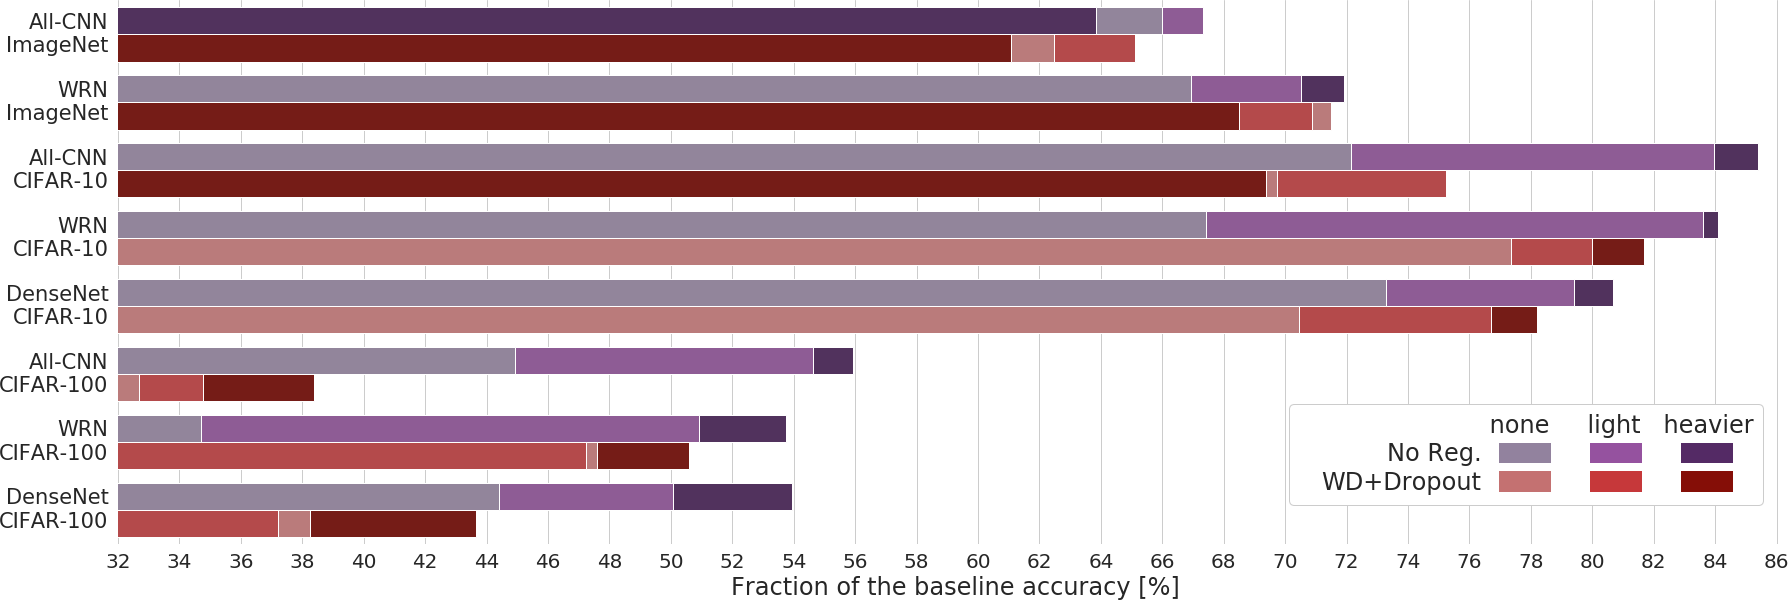
\includegraphics[keepaspectratio=true, width=\columnwidth]{\imgpath/reduced_data_10.png}
      \caption{10~\% of the available training data}
	  \label{fig:daugreg-less_data_10}
  \end{subfigure}
  \caption{Fraction of the baseline performance when the amount of available training data is reduced, $accuracy/baseline * 100$. The models trained wit explicit regularisation present a significant drop in performance as compared to the models trained with only data augmentation. The differences become larger as the amount of training data decreases.}
  \label{fig:daugreg-less_data}
\end{figure}

We argue that one of the main drawbacks of explicit regularisation techniques is their poor adaptability to changes in the conditions with which the hyperparameters were tuned. To test this hypothesis and contrast it with the adaptability of data augmentation, we extended the analysis by training the same networks with fewer examples. All models were trained with the same random subset of data and evaluated in the same test set as the previous experiments. In order to better visualise how well each technique resists the reduction of training data, in Figure~\ref{fig:daugreg-less_data} we show the fraction of baseline accuracy achieved by each model when trained with 50~\% and 10~\% of the available data. In this case, the baseline is thus each corresponding model trained with the complete data set. Table~\ref{tab:daugreg-less_data} summarises the mean and standard deviation of each combination and Figure~\ref{fig:daugreg-bootstrap_less_data} shows the result of the bootstrap analysis.

\begin{table}[htb]
  \begin{center}
    \begin{tabular}{rcc}
      & \multicolumn{2}{c}{50~\% of the training data}    \\
      \cline{2-3} 
              & No explicit reg. & Weight decay + dropout \\
      None    & 88.11 (6.27)     & 83.20 (9.83)           \\
      Light   & 91.47 (4.31)     & 88.27 (7.39)           \\
      Heavier & 91.82 (4.63)     & 89.28 (6.63)           \\
      \vspace{-7pt}\\
      & \multicolumn{2}{c}{10~\% of the training data}    \\
      \cline{2-3} 
              & No explicit reg. & Weight decay + dropout \\
      None    & 58.72 (14.93)    & 58.75 (16.92)          \\
      Light   & 67.55 (14.27)    & 60.89 (18.39)          \\
      Heavier & 68.69 (13.61)    & 61.43 (15.90) 
    \end{tabular}
  \end{center}
  \caption{Average fraction of the original accuracy of each corresponding combination of data augmentation level and presence of weight decay and dropout.}
  \label{tab:daugreg-less_data}
\end{table}

\begin{figure}[ht]
  \centering
  \begin{subfigure}{\linewidth}
      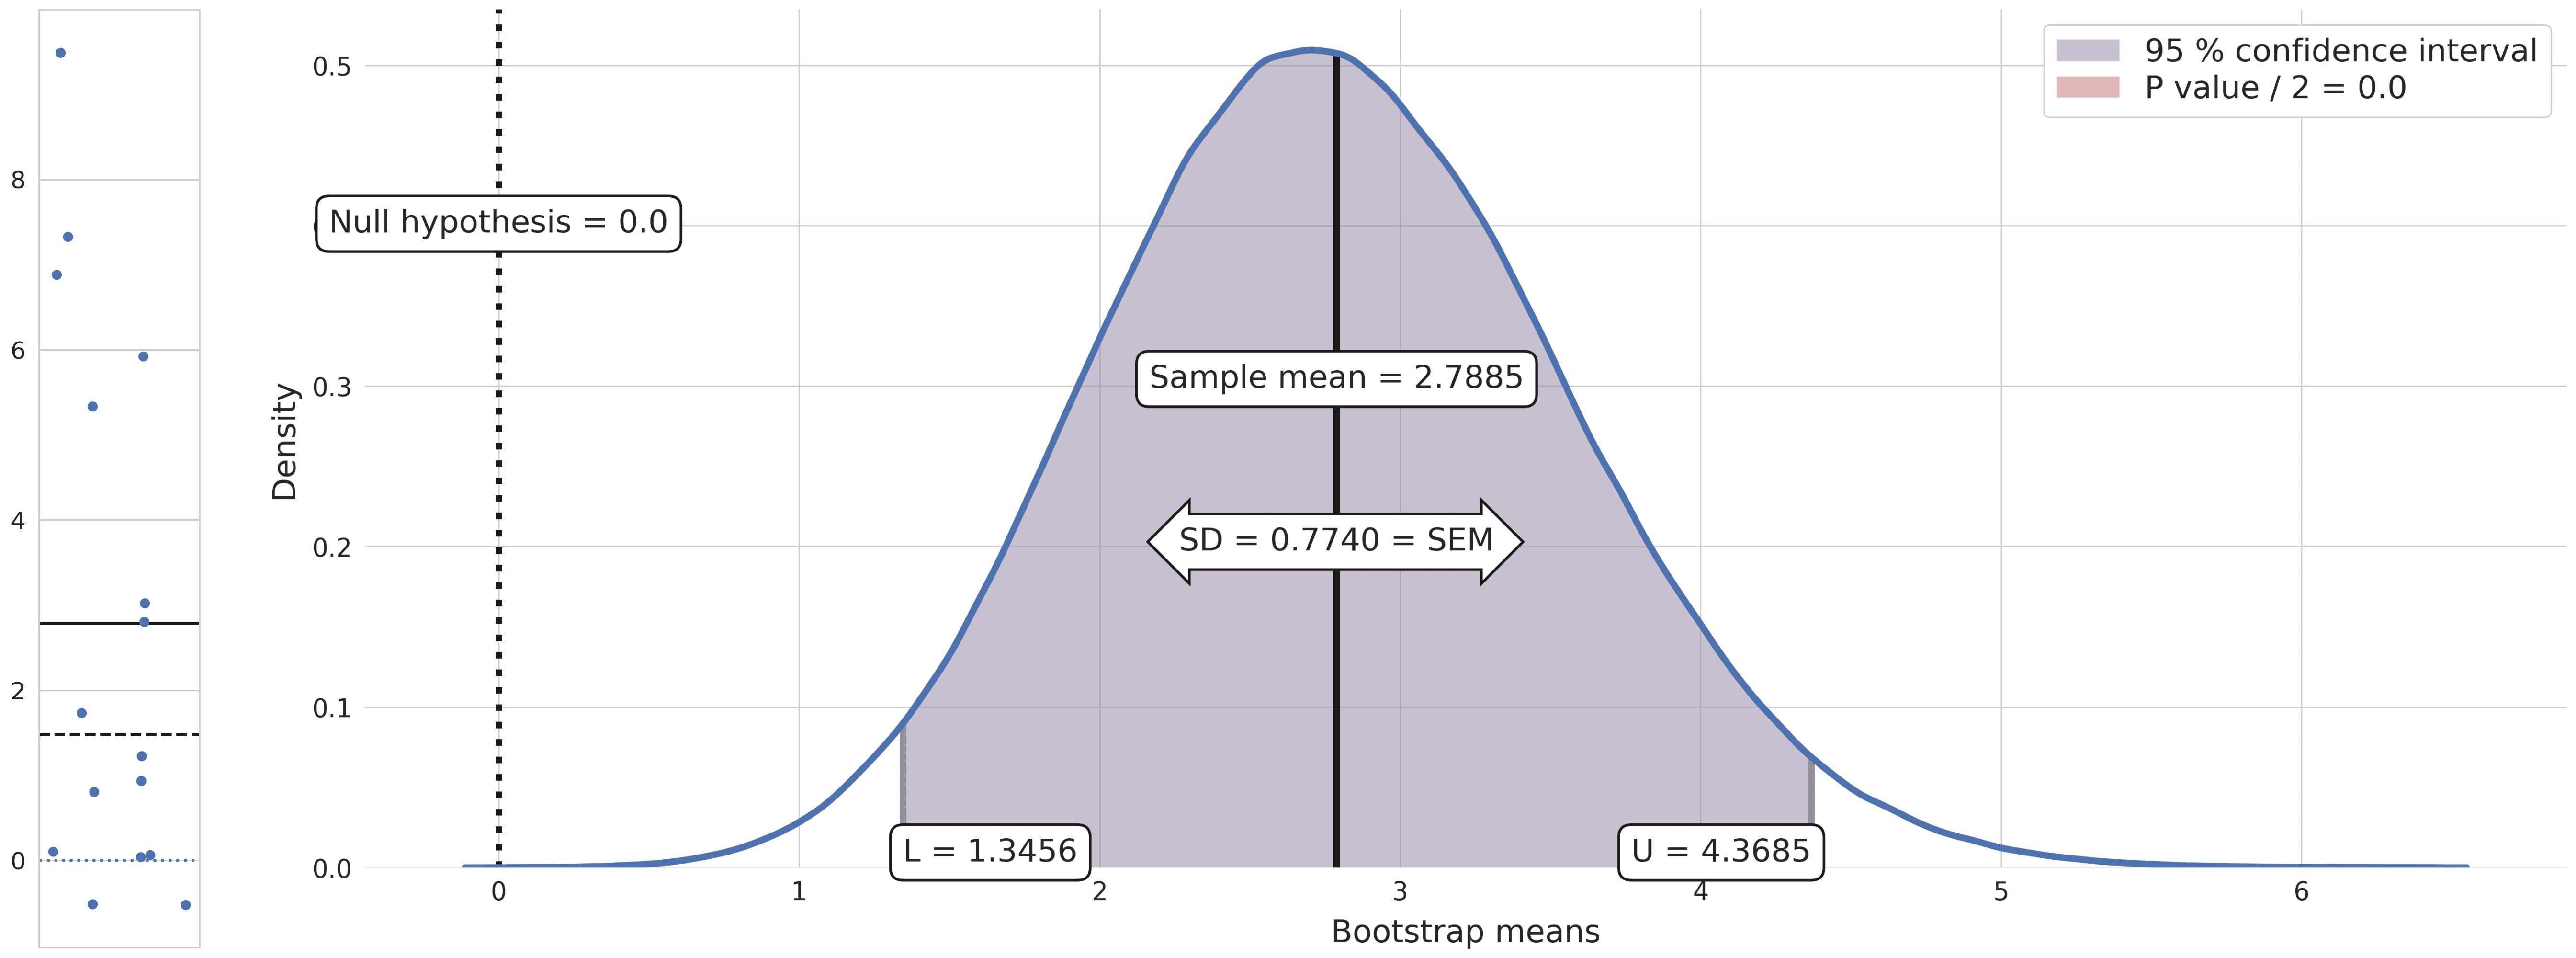
\includegraphics[width = \textwidth]{\imgpath/bootstrap_50.png}
      \caption{50~\% of the available training data}
      \label{fig:daugreg-bootstrap_means_50}
  \end{subfigure}
  \\
  \begin{subfigure}{\linewidth}
      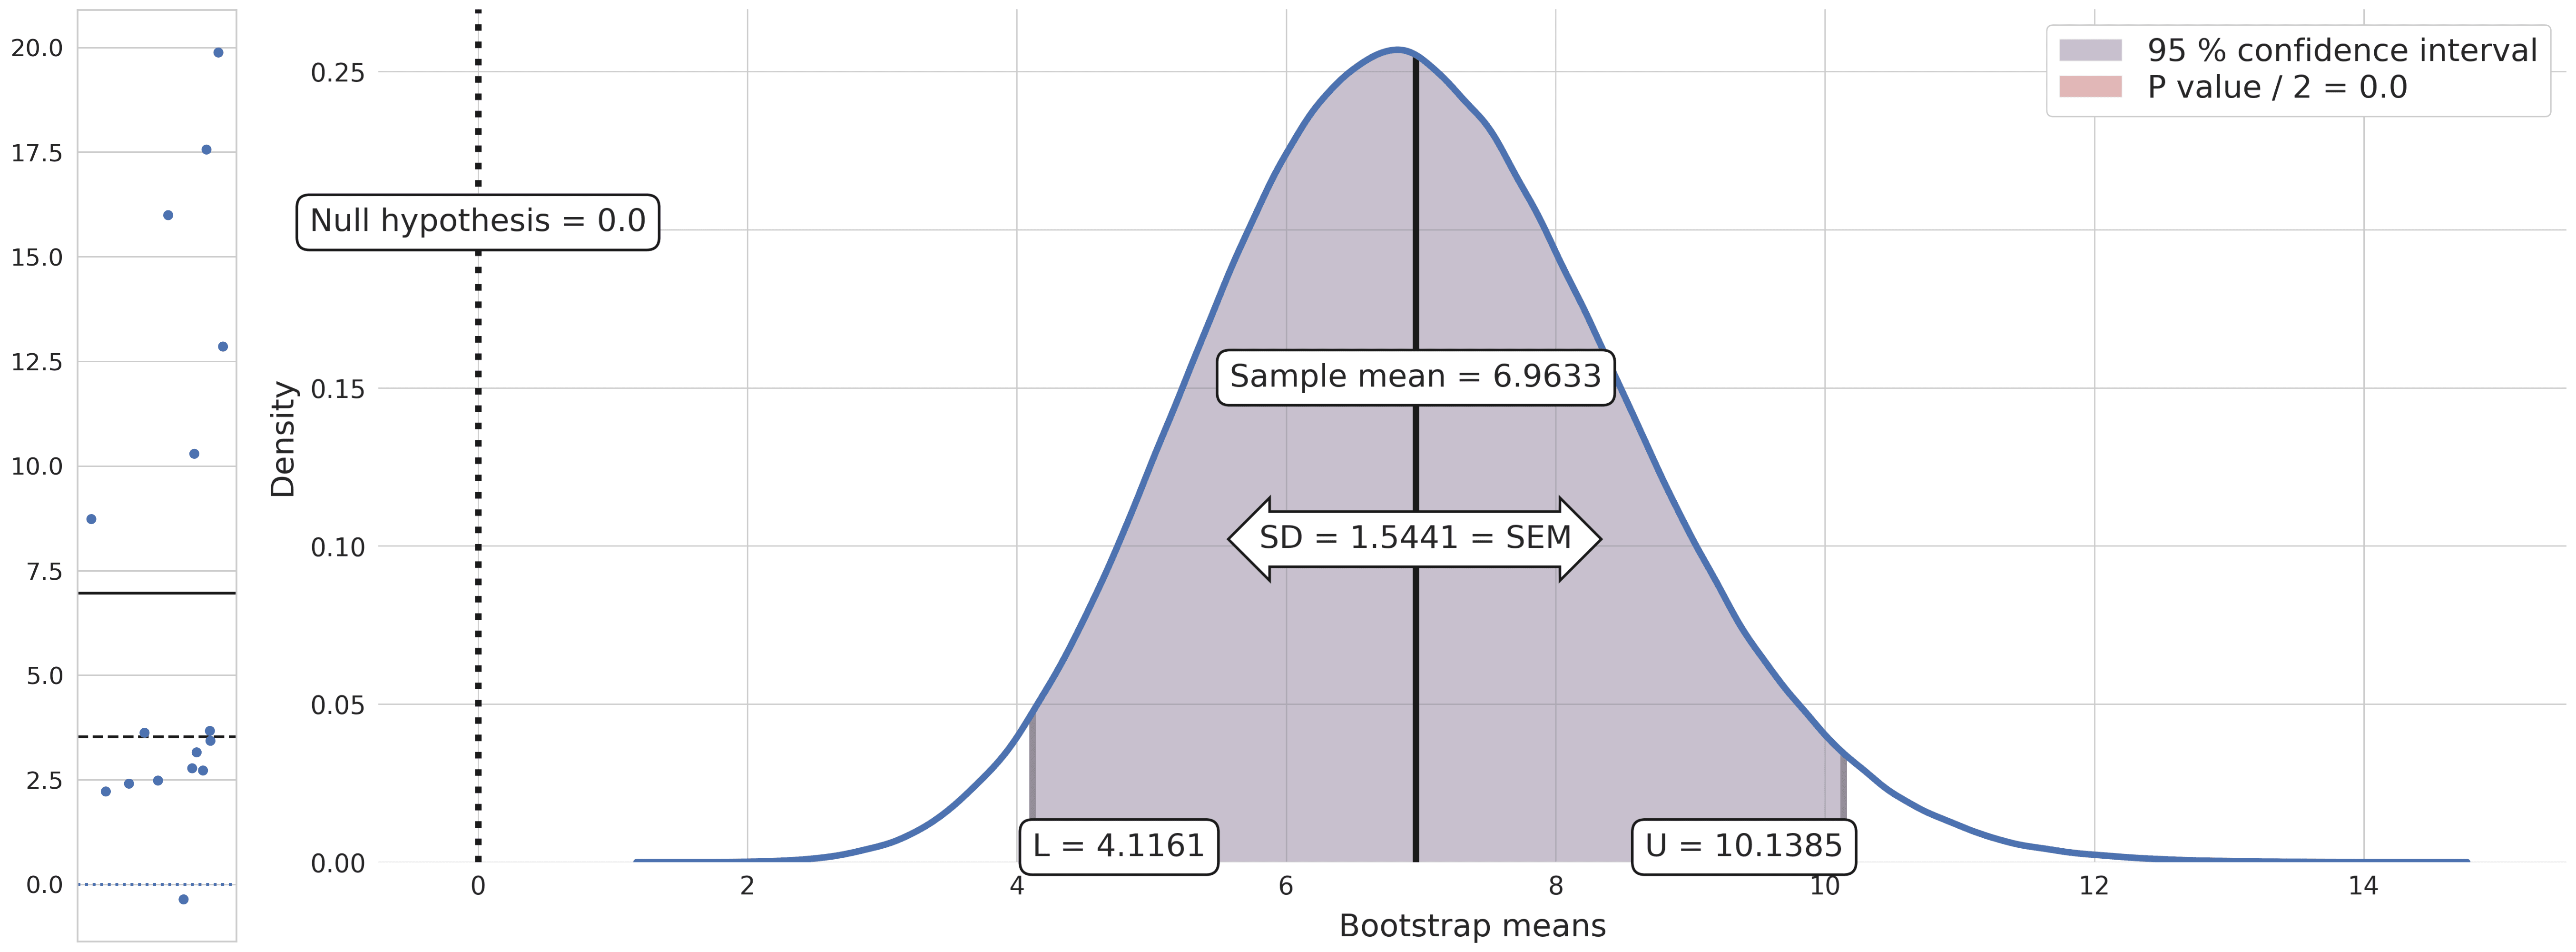
\includegraphics[width = \textwidth]{\imgpath/bootstrap_10.png}
      \caption{10~\% of the available training data}
      \label{fig:daugreg-bootstrap_means_10}
  \end{subfigure}
  \caption{Bootstrap analysis analogous to the one detailed in Section~\ref{sec:daugreg-orig} and Figure~\ref{fig:daugreg-bootstrap_orig}, to analyse the statistical significance of the performance difference of models trained with only 10 and 50~\% of the data.}
  \label{fig:daugreg-bootstrap_less_data}
\end{figure}

One of the main conclusions of this set of experiments is that if no data augmentation is applied, explicit regularisation hardly resists the reduction of training data by itself. On average, with 50~\% of the available data, these models only achieve 83.20~\% of the original accuracy (Table~\ref{tab:daugreg-less_data}), which, remarkably, is even worse than the models trained without any explicit regularisation (88.11~\%). On 10~\% of the data, the average fraction is the same (58.75 and 58.72~\%, respectively). This implies that training with explicit regularisation is even detrimental for the performance.

When combined with data augmentation, the models trained with explicit regularisation (bottom, red bars) also perform worse (88.78 and 61.16~\% with 50 and 10~\% of the data, respectively), than the models without explicit regularisation (top, purple bars, 91.64 and 68.12~\% on average). Note that the difference becomes larger as the amount of available data decreases. Even more decisive are the results of the bootstrap analysis (Figure~\ref{fig:daugreg-bootstrap_less_data}): the mean difference of the fraction of the performance achieved by the models trained without and with explicit regularisation is 2.78 and 6.96, with 50 and 10~\% of the training data, respectively; the confidence intervals are well above the null hypothesis and the $P$ values are exactly 0.

Importantly, it seems that the combination of explicit regularisation and data augmentation is only slightly better than training without data augmentation. Two reasons may explain this: first, the original regularisation hyperparameters seem to adapt poorly to the new conditions. The hyperparameters were specifically tuned for the original setup and they would require re-tuning to obtain comparable results. Second, since explicit regularisation reduces the representational capacity, this might prevent the models from taking advantage of the augmented data.

In contrast, the models trained without explicit regularisation but with data augmentation more naturally adapt to the reduced availability of data. With 50~\% of the data, these models achieve about 91.5~\% of the performance with respect to training with the complete data sets. With only 10~\% of the data, they achieve nearly 70~\% of the baseline performance, on average. This highlights the suitability of data augmentation to serve, to a great extent, as true, useful data \citep{vinyals2016oneshot}.

\subsection{When the architecture changes}
\label{sec:daugreg-depth}
\begin{figure}[tb]
  \begin{center}
    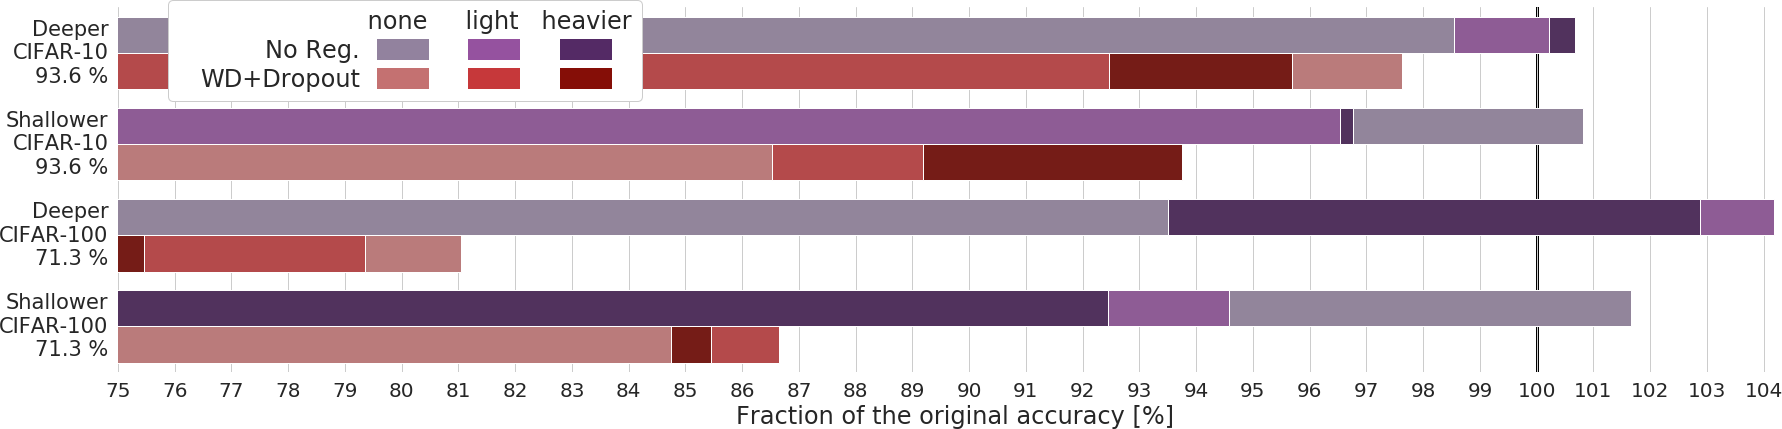
\includegraphics[width = \linewidth]{\imgpath/diff_depth.png}
  \end{center}
  \caption{Fraction of the original performance when the depth of the All-CNN architecture is increased or reduced in 3 layers. In the explicitly regularised models, the change of architecture implies a dramatic drop in the performance, while the models trained without explicit regularisation present only slight variations with respect to the original architecture.}
  \label{fig:daugreg-depth}
\end{figure}

Finally, in the same spirit, we tested the adaptability of data augmentation and explicit regularisation to changes in the depth of the All-CNN architecture, by training shallower (9 layers) and deeper (15 layers) versions of the architecture. We show the fraction of the performance with respect to the original architecture in Figure~\ref{fig:daugreg-depth} and the bootstrap analysis in Figure~\ref{fig:daugreg-bootstrap_depth}.

\begin{figure}[ht]
  \begin{center}
    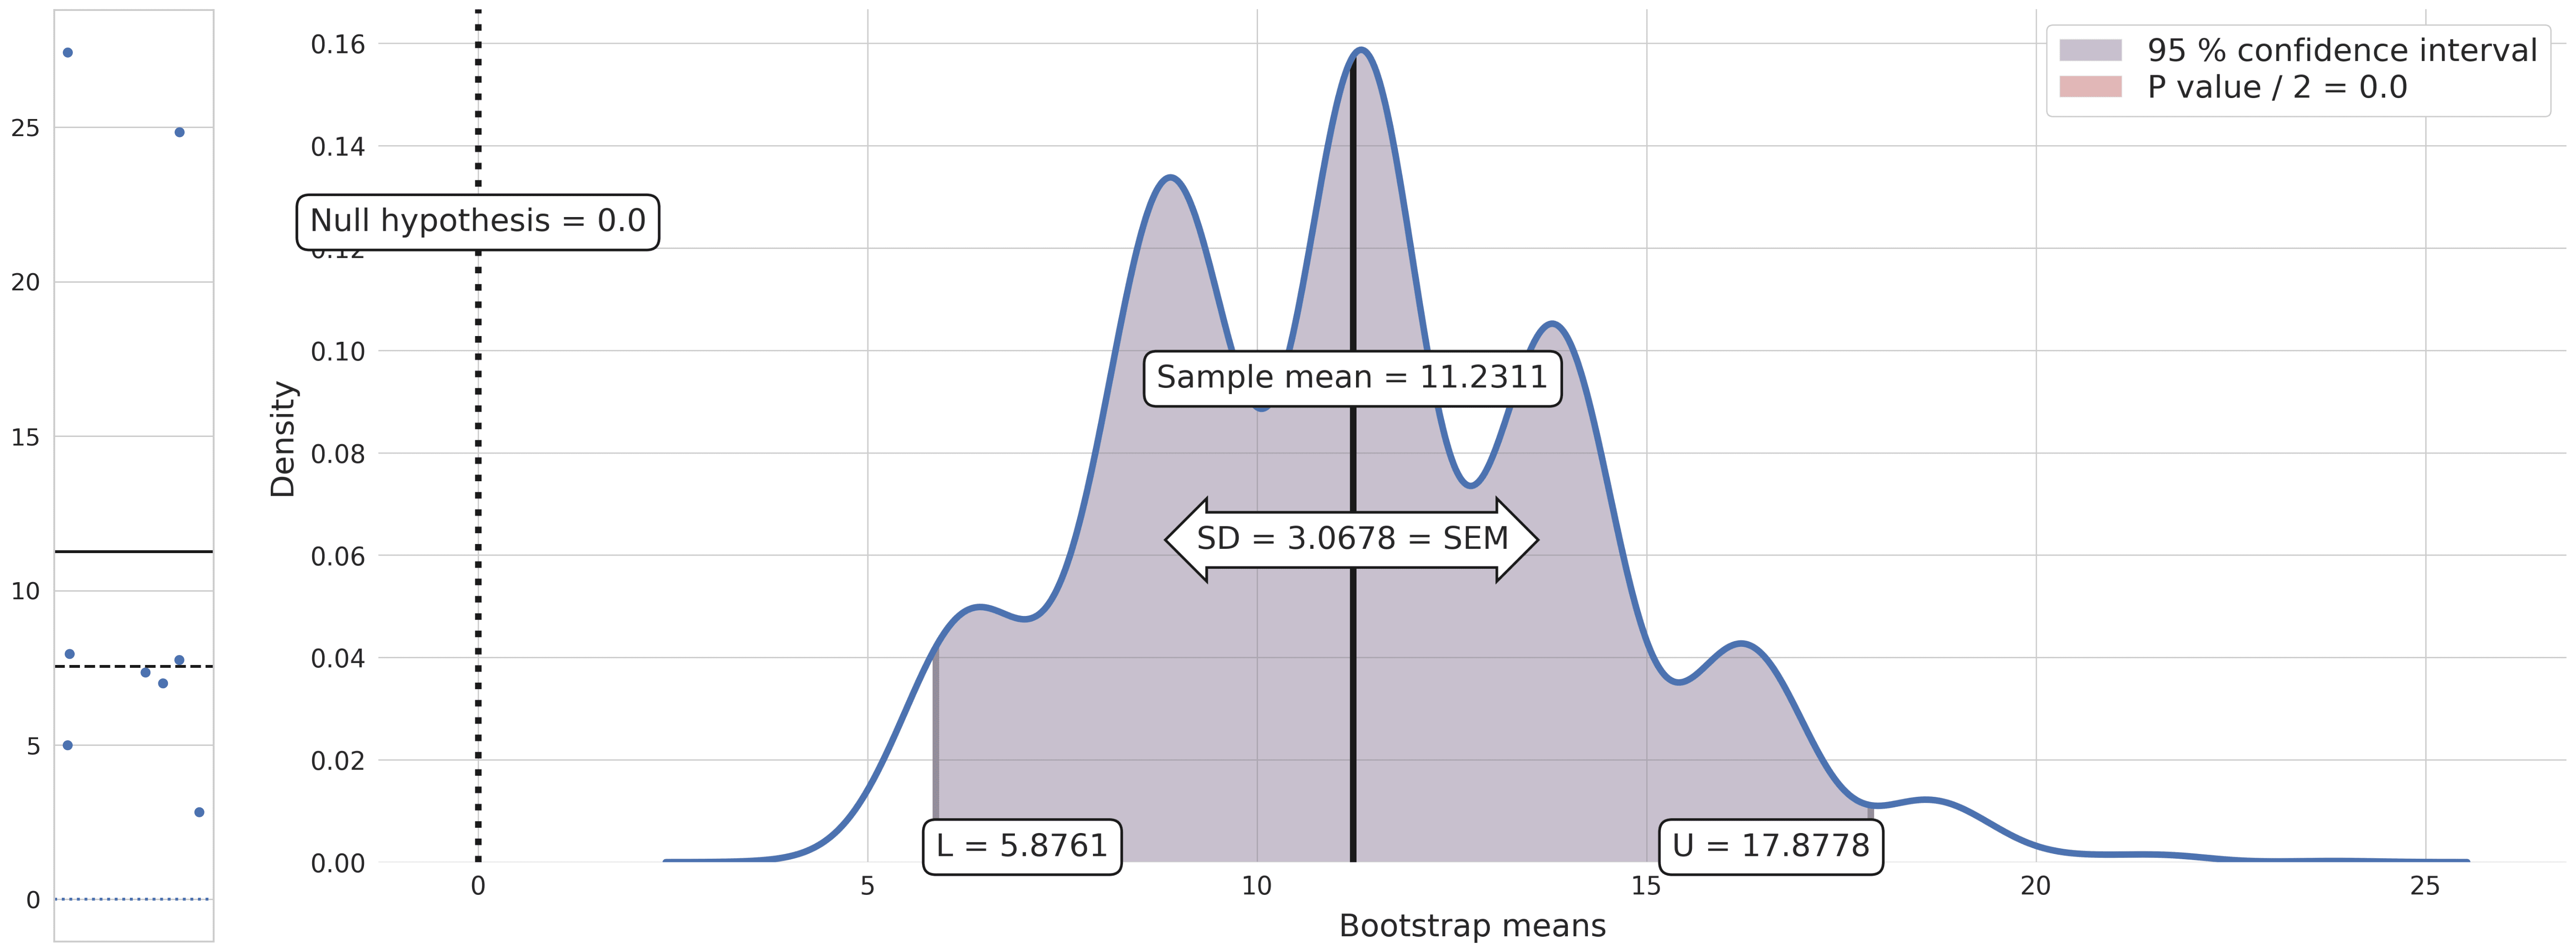
\includegraphics[width = \textwidth]{\imgpath/bootstrap_depth.png}
  \end{center}
  \caption{Bootstrap analysis analogous to the one detailed in Section~\ref{sec:daugreg-orig} and Figure~\ref{fig:daugreg-bootstrap_orig}, to analyse the statistical significance of the performance difference of All-CNN trained with 3 more and 3 fewer layers.}
  \label{fig:daugreg-bootstrap_depth}
\end{figure}

A noticeable result from these experiments is that all the models trained with weight decay and dropout (bottom, red bars) suffered a dramatic drop in performance when the architecture changed, regardless of whether deeper or shallower and of the amount of data augmentation. As a matter of fact, the models trained without explicit regularisation performed on average 11.23~\% ($SD = 3.06$) better. As in the case of reduced training data, this may be explained by the poor adaptability of the regularisation hyperparameters, which strongly depend on the architecture.

This highly contrasts with the performance of the models trained without explicit regularisation (top, purple bars). With a deeper architecture, these models achieve slightly better performance, effectively exploiting the increased capacity. With a shallower architecture, they achieve only slightly worse performance\footnote{Note that the shallower models trained with neither explicit regularisation nor data augmentation achieve even better accuracy than their counterpart with the original architecture, probably due to the reduction of overfitting provided by the reduced capacity.}. Thus, these models seem to more naturally adapt to the new architecture and data augmentation becomes beneficial.

It is worth commenting on the particular case of the CIFAR-100 benchmark, where the difference between the models with and without explicit regularisation is even more pronounced, in general. It is common practice in object recognition papers to tune the parameters for CIFAR-10 and then test the performance on CIFAR-100 with the same hyperparameters. Therefore, these are typically less suitable for CIFAR-100. We believe this is the reason why the benefits of data augmentation seem even more pronounced on CIFAR-100 in our experiments.

In sum, these results highlight another crucial advantage of data augmentation: the effectiveness of its hyperparameters, that is the type of image transformations, depend mostly on the type of data, rather than on the particular architecture or amount of available training data, unlike explicit regularisation hyperparameters. Therefore, removing explicit regularisation and training with data augmentation increases the flexibility of the models.

\section{Discussion}
\label{sec:daugreg-discussion}
In this section we summarise our findings and discuss their relevance. In particular, we challenge the need for weight decay and dropout to train artificial neural networks, and propose to rethink data augmentation as a \textit{first class} technique instead of a \textit{cheating} method.

As an empirical analysis, one caveat of our work is the limited number of experiments (over 300 models trained). In order to increase the generality of our conclusions, we chose three significantly distinct network architectures and three data sets. Importantly, we also took a conservative approach in our experimentation: all the hyperparameters were kept as in the original models, which included both weight decay and dropout, as well as light augmentation. This setup is clearly suboptimal for models trained without explicit regularisation. Besides, the heavier data augmentation scheme was deliberately not optimised to improve the performance as it was not the scope of this work to propose a specific data augmentation technique. We leave for future work to explore data augmentation schemes that can more successfully be exploited by any deep model. Finally, in order to strengthen the conclusions from the empirical analysis, we have also discussed some theoretical insights in Section~\ref{sec:daugreg-theoretical_insights}, concluding that the generalisation gain provided by weight decay can be seen as a lower bound of what can be achieved by domain-specific data augmentation. We also hope that this work inspires researchers in other application domains, such as natural language processing, to further contrast data augmentation and explicit regularisation.

\subsection{Do deep nets really need weight decay and dropout?}
\label{sec:daug_vs_reg-wd_drop}
In Section~\ref{sec:daugreg-results} we have presented the results of a systematic empirical analysis of the role of weight decay, dropout and data augmentation in deep convolutional neural networks for object recognition. Our results have shown that explicit regularisation is not only unnecessary \citep{zhang2016understandingdl}, but also that its performance gain can be achieved by data augmentation alone: in most cases, training with data augmentation only was better than training with both data augmentation and explicit regularisation. In the few cases where that was not the case, the difference was very small. Moreover, unlike data augmentation, models trained with weight decay and dropout exhibited poor adaptability to changes in the architecture and the amount of training data. Why do researchers and practitioners keep training their neural networks with weight decay and dropout? Do deep nets really need weight decay and dropout?

The relevance of these findings lies in the fact that weight decay and dropout are almost ubiquitously present in convolutional neural networks \citep{huang2017densenet, zagoruyko2016wrn, springenberg2014allcnn}, including recent, state of the art models \citep{tan2019efficientnet}. Certainly, it has been shown in multiple research papers that weight decay and dropout can boost the performance of neural networks, and we here do not challenge the usefulness of weight decay and dropout, but the convenience to use it, given the associated cost and risk, and available alternatives. 

First, not only add weight decay and dropout extra computations during training, but also they typically require training the models several times with different hyperparameters: the coefficient of the penalty for weight decay; for dropout, the location of the dropout mask and the amount of units to drop. These hyperparameters are arguably very sensitive to changes in elements of the learning process. Here we have studied changes in the amount of training data (Section~\ref{sec:daugreg-less_data}) and the depth of the architecture (Section~\ref{sec:daugreg-depth}). Consider, for instance, our results in Section~\ref{sec:daugreg-less_data}: All-CNN trained on CIFAR-10 with weight decay, dropout and light augmentation reaches about 92~\% accuracy. If we were in the development process and were unsure about what architecture to use, we could simply try our network with three more layers and we would obtain about 85~\% accuracy. We could also try an architecture with three fewer layers and obtain about 82~\% accuracy. This may lead us to conclude that the first architecture has the right number of layers, because adding or removing layers drastically reduces the performance; or perhaps that by adding or removing layers there is some negative interaction between the layers sizes, or any other of the many hypothesis we could think of.

Consider now what happens if we train without weight decay and dropout: All-CNN trained on CIFAR-10 with light augmentation---but without weight decay and dropout---obtains about 93.3~\% accuracy. This is slightly better than the explicitly regularised model, but we will ignore this now. If we train this model with three more layers, we obtain 93.4~\% accuracy, that is the same or slightly better---as opposed to the drop of 7 points we have seen before. If we train with three fewer layers, we obtain about 90~\% accuracy, a drop of 3 points---as opposed to a drop of 10 points. In this case, we would not conclude that adding or removing layers creates negative interactions. Note that the only difference between these two cases is that the first models are trained with weight decay and dropout. Therefore, it may be reasonable to only include explicit regularisation in the final version of a model, in order to potentially obtain a slight boost in performance prior to publication or production---provided the hyperparameters are adequately fine-tuned---but keeping weight decay and dropout as intrinsic part of our models can certainly lead us astray.

Finally, we can draw some connections between the results from this chapter and the insights from the previous chapter. In Chapter~\ref{ch:reg} we discussed that the role of explicit regularisation techniques, such as weight decay and dropout, is to reduce the representational capacity of the models. This, according to statistical learning theory, can reduce overfitting and in turn improve generalisation. However, artificial neural networks have usually orders of magnitude more parameters than training examples, and they still generalise well. While this phenomenon is still not well understood, one working hypothesis is that overparameterisation does not cause negative overfitting, but rather smooth fitting that can be suitable for accurate interpolation \citep{belkin2019biasvariance, hasson2020directfit}. If overparameterisation is not a problem for artificial neural networks, is it then necessary to constrain the representational capacity through explicit regularisation? Is it reasonable to train very large models, that require a lot of memory and computation---and negatively impact the environment---and at the same time constrain their capacity?

We also hypothesise that a reason why artificial neural networks generalise well in many tasks is due to the fact that the models include many sources of implicit regularisation or, in other words, inductive biases. For example, it is known that stochastic gradient descent naturally converges to solutions with small norm \citep{zhang2016understandingdl, neyshabur2014implicitreg}, batch normalisation also contributes to better generalisation, convolutional layers are particularly efficient to process image data---and not only---to name a few examples. In our case, we argue that data augmentation has the potential to encode very powerful inductive biases that improve generalisation. We conclude that in the presence of many other sources of implicit regularisation and more effective inductive biases, weight decay and dropout may not be necessary to train large deep artificial neural networks\footnote{Previous work has suggested interesting connections between weight decay and other types of regularisation and improved adversarial robustness \citep{galloway2018wdadversarial, jakubovitz2018regadversarial}. An interesting avenue for future work is studying whether this effects are also provided by data augmentation}.

\subsection{Rethinking Data Augmentation}
\label{sec:daugreg-rethink_daug}
Data augmentation is often regarded by authors of machine learning papers as \textit{cheating}, suggesting it should not be used in order to test the potential of newly proposed methods \citep{goodfellow2013maxout, graham2014fracmaxpool, larsson2016fractalnet}. In contrast, weight decay and dropout are considered intrinsic elements of the algorithms \citep{tan2019efficientnet}. In view of our results, we propose to rethink data augmentation and switch roles with explicit regularisation: good models should effectively exploit data augmentation and explicit regularisation should only be applied, if at all, once all other elements are fixed. This approach improves the performance and saves computational resources.

In this regard, it is worth highlighting some advantages of data augmentation: Not only does it not reduce the representational capacity, unlike explicit regularisation, but also, since the transformations reflect plausible variations of the real objects, it increases the robustness of the model \cite{novak2018sensitivity, rusak2020robustness}. Interestingly, in Chapter~\ref{ch:daugit} we will also show that models trained with heavier data augmentation learn representations more aligned with the inferior temporal (IT) cortex, highlighting its connection with visual perception and biological vision. Deep nets are especially well suited for data augmentation because they do not rely on pre-computed features. Moreover, unlike explicit regularisation, it can be performed on the CPU, in parallel to the gradient updates. Finally, from Sections~\ref{sec:daugreg-less_data} and~\ref{sec:daugreg-depth} we concluded that data augmentation naturally adapts to architectures of different depth and amounts of available training data, without the need for specific fine-tuning of hyperparameters.

A commonly cited disadvantage of data augmentation is that it depends on expert knowledge and it cannot be applied to all domains \citep{devries2017daugfeatspace}. However, we argue instead that expert and domain knowledge should not be disregarded but exploited. Expert and domain knowledge are, in fact, useful inductive biases. A remarkable advantage of data augmentation is that a single augmentation scheme can be designed for a broad family of data---for example, natural images, using our knowledge about visual perception---and effectively applied to a broad set of tasks---object recognition, segmentation, localisation, etc. We hope that these insights encourage more research on data augmentation and, in general, highlight the importance of using the available data more effectively. In the following chapters, we explore additional properties of models trained with data augmentation (Chapter~\ref{ch:daugit}) and how it can be used as part of the objective function to learn representations more aligned with the properties of the primate visual cortex (Chapter~\ref{ch:invariance}).

\chapterbibliography
}
